\documentclass[]{article}
\usepackage{graphicx}
\graphicspath{{./}{figures/}}

\begin{document}
	The IceCube Neutrino Observatory is a cubic-kilometer array buried 1.5km beneath glacier ice at the geographic south pole. When neutrinos undergo charged-current  or neutral-current interactions in the ice, daughter leptons emit Cherenkov light that can be detected by IceCube's 5160 Detector Optical Modules (DOMs). 
	In 2013, IceCube discovered a diffuse flux of high-energy astrophysical neutrinos. Since then, there has been an going search to find potential source candidates. 
	
	Auto-correlation analyses searching for steady neutrino sources, neutrino flares or coincident neutrino multiplets have so far failed to find any significant clustering within the neutrino flux. The consistency of this flux with an isotropic distribution suggests that it has a predominantly extragalactic origin. The lack of independently-identified neutrino sources has motivated targeted searches using multi-wavelength and multi-messenger data, seeking to identify an excess of neutrinos correlated with a given source or source class.
	
	In general, the sensitivity of neutrino telescopes is limited by the background flux of atmospheric neutrinos, as well as atmospheric muons, which exceed the measured astrophysical neutrino flux by orders of magnitude except at the very highest energies above O(100TeV). 
	
	This vast background can be overcome with two complementary approaches. In the neutrino-driven approach, neutrino events are selected which have a high-probability to be of astrophysical orgin, based on their reconstructed topology. For these neutrinos, possible counterparts can be identified. Such an approach forms the basis of the IceCube Realtime Program, in which likely astrophysical neutrinos are identified in real-time and immediately distributed as "alerts" to astronomers via the Gamma-ray Coordination Network (GCN) framework. Because only a handful of neutrinos are identified with these filters each year, it can be hard to make statistically-signficant statements about source populations using this approach. Furthermore, these searchers are hampered by the abundance of unresolved neutrino sources that would be expected for most source populations. For example, in X, it was highlighted that for a CCSN-like population of neutrino sources, only ~20 \% of all astrophysical neutrinos would be expected to have resolvable counterparts. Given a neutrino alert stream of 50 \% purity, this would require 10 sucessful follow-up campaigns before a single coincidence was identified.
	
	In the alternative source-driven approach, specific source hypotheses are tested. These searches typically exploit the large expected number of lower-energy astrophysical neutrinos, enabling analysis with significantly higher statistics at the cost of greater atmospheric background. Requiring spatial coincidence with a potential source does, however, significantly reduce the background for a search. Another effective method is to additionally require temporal coincidence, either with the lifetime of a transient, or during  pre-defined "interesting periods" for variable objects. Multiple sources can be combined in a stacking analysis, which are designed to detect the sum of many weak individual sources. In all cases, these methods rely on multi-messenger and multi-wavelength observations to identify sources to be analysed.
	
	The most sucessful example of the neutrino-driven approach followed the detection of a high-energy neutrino in September 2017. Following the automated alert generated by this neutrino,  IC170922A, a comprehensive multi-messenger follow-up campaign was launched. The Fermi collaboration reported that the neutrino was coincident with a flaring gamma-ray blazar, and subsequent observations by the MAGIC collaboration revealed Very-High Energy (VHE) gamma-ray emission. A chance coincidence of this kind was disfavoured at the level or 3$\sigma$.
	
	At the same time, previous IceCube analysis has limited the cumulative distribution of Fermi blazars to the astrophysical neutrino flux to be less than ~30\%. The origin of the vast majority of the diffuse neutrino flux thus remains, as yet, undiscovered. Dedicated searches targeting likely sources, including Gamma-Ray Bursts (GRBs), Core-Collapse Supernovae(CCSNe), Starburst galaxies and galactic emission, have so far failed to reveal any significant excess above background expectations. This motivates the continued analysis of new, untested source classes in an attempt to identify the origin of astrophysical neutrinos.
	
	Within this context, a new analysis was undertaken to search for neutrinos from Tidal Disruption Events (TDEs). A TDE occurs when a star approaches a supermassive black hole (SMBH) on a parabolic orbit. As gravitational acceleration follows a $\frac{1}{r^{2}}$ dependence, the near side of the star will be accelerated more strongly than the far side. The star thus experiences a net tidal force. As the star moves closer to the SMBH, the tidal forces increases, until it exceeds the self-gravity that holds the star together. At this point, the star is said to be tidally-disrupted, and roughly half of the stellar debris is accreted. In some cases, a relativstic jet can be formed during the accretion process, analagously to a blazar jet. There has been recent theoretical interest in TDEs as potential Ulta-High Energy Cosmic Ray (UHECR) sources, as well as candidate neutrino sources (Y, Z).
	 
	TDEs are a fundamentally rare phemomenon, with rates several orders of magnitude below CCSN rates (SJOERT). However, historically poor detection efficiences have further exacerbated this, leaving only a handful of reliably-identified TDEs. To date, there have been only 3 on-axis Jetted TDEs (ABC), and a few dozen candidate non-jetted TDEs. Of these, the majority do not have an unambiguous TDE classification. 
	
	TDEs themselves are, by their nature, nuclear transients. They can often be confused with flares of Active Galactic Nucleii (AGN), as well as nuclear CCSNe. Due to the greater abundance of these background populations, it can be hard to remove all contamination. Ultimately muliple eras of spectroscopy and photometry are required for a compelling classification. At the time of catalogue compilation in October 2017, out of approximately 60 candidate TDEs in the literature, only 13 could be reliably classified. 
	
	The stacking method employed for the analysis did not make assumptions on the relative strength of each tested source, and was thus robust against both catalogue contamination and deviations from a standard-candle neutrino emission scheme. However, in order to meaningfully interpret the results, and extrapolate to constrain emission from the population as a whole, a pure sample is required. 
	
	\begin{figure}[!ht]
		\centering 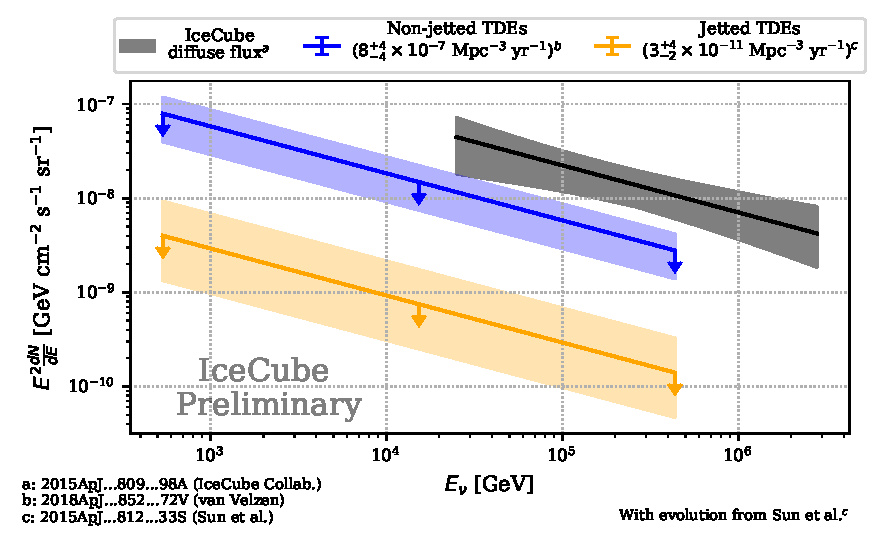
\includegraphics[width=\textwidth]{figures/diffuse_flux_global_fit}
		\caption{Limits on the contribution of jetted and non-jetted TDEs to the diffuse neutrino flux. The shaded bands represent uncertainty in local rate estimates.}
		\label{fig:DiffuseFlux}
	\end{figure}
	
	Consequently, the non-jetted sample was separated based on robustness of classification, with the "Golden TDEs" being assumed representative of non-jetted TDEs as a whole. The results are shown in Figure \ref{fig:DiffuseFlux}. Assuming central rate estimates from Y and X, we find that Jetted and Non-Jetted TDEs contribute less than 26\% and 1.3\% respectively to the astrophysical neutrino flux. As the contribution from a population is directly proportional to the local population rate, the shaded bands indicate the uncertainty in our limits arising from rate estimates.
	
	For TDEs, these rates are the dominant source of uncertainty in neutrino flux. It will require systematic evaluation of observed TDE rates to enable more precise limits on neutrino emission. Any refined rate estimate can be immediatly used to diretly recalculate  limits, without requiring any additional IceCube analysis.
	
	The discovery of extraordinary transient AT2018cow was a further demonstration of the central importance of multi-messenger observations.  This fast, bright, blue transient prompted a comprehensive multi-messenger follow-up campaign, and was variously interpreted as a TDE, an extreme SN or a Magnetar. The observations were consistent with a nearby example of a recently-identified population of Fast Blue Optical Transients (FBOTs). A new analysis of AT2018cow, extending from 30 days before peak to 100 days afterwards, did not reveal any significant neutrino emission. The correpsonding constraints are illustrated in Figure \ref{fig:At2018cow}. As before, uncertainty in both classification and rate estimates hinder attempts to constrain neutrino emission from FBOTs.
	
	\begin{figure}[!ht]
		\centering 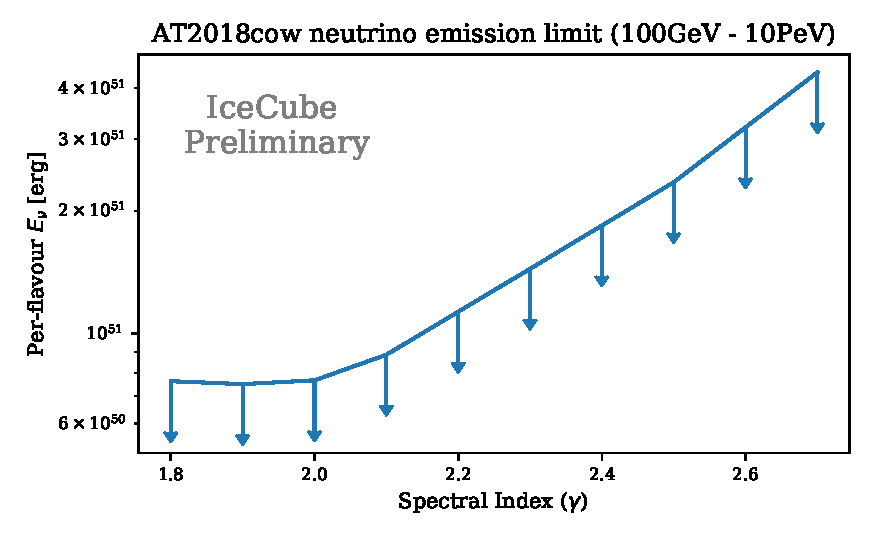
\includegraphics[width=\textwidth]{figures/AT2018cow_limit_plot}
		\caption{Limits on integrated neutrino emission from AT2018cow as a function of spectral index, assuming a 130 day window from X to Z.}
		\label{fig:At2018cow}
	\end{figure}
	
	Fortunately, the emergence of new facilities such as ZTF, as well as future surveys such as LSST, should greatly aid such analyses. By discovering larger numbers of transients, the sensitivity of searches will grow. Larger samples should also improve rate estimation. Higher cadence observations can greatly reduce background by constraining search windows, for example the estimated CCSN explosion time, with greater precision. Consequently, source-driven analysis will continue to grow more powerful.
	
	
\end{document}